
As outlined in Section~\ref{sec:introduction}, we refer by trending to the consistency of an observed change with the change issued by another measurement, a nowcast, or a forecast.
In this section, we want to specify trending and lay out different methods of measuring and visualizing trending. 
In general, trending can be assessed for different lags $l$ separately, and the relevance of considered lags has to be determined based on the question at hand.
Throughout the section, we call a measurement, nowcast, or forecast a \textit{prediction} or \textit{signal}.
Before introducing measures for assessing trending, we give remarks on computing the predicted change and notation in Section~\ref{subsec:notation}.
The remainder of the section is structured as follows.
Section~\ref{subsec:trending-basics} introduces trending basics and visualizes trending in a synthetical example.
Section~\ref{subsec:trending-measures} reviews conveyed quantification approaches from other fields.
The approaches are extended to the trending setting in Section~\ref{subsec:trending-noise}.
Section~\ref{subsec:trending-cond-prob} introduces a new graphical method of trending assessment and briefly introduces bootstrap methods for computing confidence intervals for the measures.

\subsection{Computing the predicted change and notation}\label{subsec:notation}

As noted above, trending refers to observed and predicted changes for a time lag $l$.
The observed change is straightforward to compute for measurements, nowcasts, and forecasts.
Let $\mathbf{y} = (y_t)_{t=0}^T$ denote the true values or gold standard measurements up to time $T$.
The sequence of observed change is then given by the differences of values in $\mathbf{y}$ with lag $l$, that is
\begin{equation}\label{eq:diffy}
    \diffylt = (y_{t+l} - y_t) \quad \text{for}\ t = 1, \dots, T - l.
\end{equation}
As noted in the introduction, the definition of predicted change depends on the context.
Conveying the computation for $y$ directly, the signal's predicted change would be the difference between the signal at time $t + l$ and the true value at $t$.
This approach lags in three practical aspects.
For nowcasting and forecasting, the true value at time $t$ might not be known with a considerable time lag.
In the example in Section~\ref{sec:application-covid}, for example, the time lag is more than 80 days.
Until the true values are publicly available, the change cannot be computed, and no actions can be taken based on it.
Thus, it is more practically relevant to use updated signal values for time $t$ as the reference value in this setting.

Second, in the context of nowcasting or forecasting, several signals for the same time $t + l$ are often available at different generation times.
Thus, it has to be specified in notation which signal generated at which time is used.
We use the term \textit{issue time} for the generation time of a signal and \textit{target time} to denote the time the forecast applies to.

For measurement, a test method is usually evaluated against a gold standard to test whether the test method could replace the gold standard.
If the test method is assessed to be consistent with the gold standard, the gold standard measurement values are not available to compute the predicted change.
Thus, the predicted change is computed based on the test method's values at time $t$ and $t + l$.

Taking the three points together, the signal's predicted change is based on the type of signal.
To account for several signals for a forecast time $t$ at different issue times $\tau$, we denote those by $x_{t | \tau}$.
For nowcasting, $t$ and $\tau$ are usually close and possibly negative; for forecasting, $t$ is usually larger than $\tau$.
For measurements, this distinction is not necessary.
Table~\ref{tab:notation} summarizes the notation for the different signal types and the predicted change computation.

\begin{table}
    \centering
    \begin{tabularx}{0.75\textwidth}{l X}
        \toprule
        Application & Predicted change computation \\
        \midrule
        Measurement & $(x_{t + l} - x_t)_{t=0}^T \label{eq:diffxl_measure} $\\
        Nowcasting & $
\diffxl =
\begin{cases}
(x_{t+l|t+l} -x_{t|t+l})^T_{t=0} & \text{if } y_{t} \text{ is not known at time } t, \\
(x_{t+l|t+l} -y_{t})^T_{t=0} & \text{else}.
\end{cases} \label{eq:diffxl_nowcasting}
$ \\
        Forecasting & $
\diffxl =
\begin{cases}
(x_{t+l|t} - x_{t|t})^T_{t=0} & \text{if } y_{t} \text{ is not known at time } t, \\
(x_{t+l|t} - y_{t})^T_{t=0}  & \text{else}.
\end{cases} \label{eq:diffxl_forecasting}
$\\
        \bottomrule
    \end{tabularx}
    \caption{Computation of the predicted change in the different applications. The signals $x_{t | \tau}$ refer to values issued at $\tau$ with a target time $t$. Note the different relations of issue and target time for nowcasts and forecasts. }
    \label{tab:notation}
\end{table}


\subsection{Basics of trending and four-quadrant plots}\label{subsec:trending-basics}

Throughout the remainder of the section, we use the notation of differences, $\diffxl$ and $\diffyl$.
While the computation of $\diffx$ differs in different contexts, the trending assessment is similar.
In the following, we omit the difference's lag $l$ for the ease of notation; $\diffx$ and $\diffy$ refer to $\diffxl$ and $\diffyl$ for a common lag $l$.
As noted above, a signal is trending perfectly if all occurred directions of change are predicted correctly; that is, the sign of all elements of $\diffx$ and $\diffy$ coincide.
Perfect trending is hardly the case in practice, but a weaker requirement is needed.
Accordingly, when assessing the trending, we examine the statistical consistency of $\sign(\diffx)$ and $\sign(\diffy)$.
A simple yet insightful method is the four-quadrant plot.
For example, it is known in cardiac output measurement analysis~\parencite{Saugel2015,perrino1998intraoperative}. 
Thereby, the occurred changes are plotted together with the predicted changes, that is, $(\diffy_t, \diffx_t)$ for $t = 1, \dots, T$.
Thus, the x-axis of a four-quadrant plot shows the true value differences, whereas the y-axis displays prediction data differences.
Points in the green upper right and lower left quadrants reflect a correct trending for the respective time step, whereas points in the remaining red quadrants show incorrect predicted changes.
Figure~\ref{fig:trending_basic_4q} displays a basic four-quadrant plot.
Points 2, 3, 5, and 6 show trending, whereas points 1, 4, and 7 count for anti-trending behavior.
Figure~\ref{fig:trending_basic_4q_sample} shows a four-quadrant plot for a more extensive simulated data set with $T=1461$, for example, four years of daily data.
The data generation is described in Appendix~\ref{subsec:app-trending-data-generation} and will carry through this section.
The four-quadrant plot resembles a butterfly-like shape, with more data in the upper right and lower left quadrants than in the remaining quadrants.
The four-quadrant plot is intuitive to interpret, and the magnitude and direction of change are shown simultaneously.
It can be extended by including information on the date of difference in the point color.
In Figure~\ref{fig:trending_basic_4q_sample_color}, blue points refer to earlier measurements and turn green for larger $t$.
The lag is always one time step.
However, four-quadrant plots become crowded for larger datasets, and the sequential information on the differences is complex to assess thoroughly.
There are other visualization techniques, such as polar plots or the Bland-Altmann analysis.
However, they lack the clearness and intuition of the four-quadrant plot while adding no more information on the trending~\parencite{Saugel2015}.

\begin{figure}
\centering
\begin{subfigure}[t]{.24\textwidth}
\includegraphics{plots/illustrative_examples/4Q_without_excl}
\caption{Basic four-quadrant plot.} \label{fig:trending_basic_4q}
\end{subfigure}\hspace{0.01\textwidth}%
\begin{subfigure}[t]{.24\textwidth}
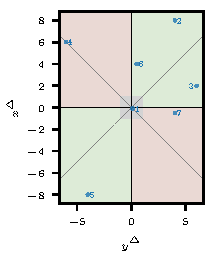
\includegraphics{plots/illustrative_examples/4q_excl_box}
\caption{Four-quadrant plot with rectangle exclusion area.}\label{fig:trending_basic_4q_excl_box}
\end{subfigure}\hspace{0.01\textwidth}%
\begin{subfigure}[t]{.24\textwidth}
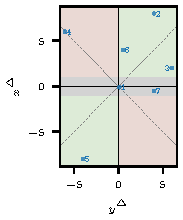
\includegraphics{plots/illustrative_examples/4q_excl_axis}
\caption{Four-quadrant plot with horizontal exclusion area.} \label{fig:trending_basic_4q_excl_axis}
\end{subfigure}\hspace{0.01\textwidth}%
\begin{subfigure}[t]{.24\textwidth}
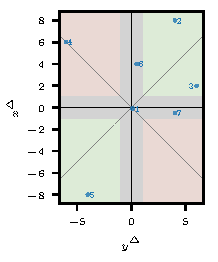
\includegraphics{plots/illustrative_examples/4q_excl_cross}
\caption{Four-quadrant plot with crossed exclusion area.}\label{fig:trending_basic_4q_excl_cross}
\end{subfigure}%
\caption{Illustrations of the four-quadrant plot with sample points and with and without exclusion areas. }
\label{fig:trending_4q}
\end{figure}

\subsection{Trending ratio and other measures}\label{subsec:trending-measures}

Analyzing the number of points in the green quadrants versus the red quadrants boils down to assessing the probability of trending $P(\diffxrv \diffyrv > 0)$, where $\diffyrv$ and $\diffxrv$ denote random variables for future incremental changes, respectively.
Note that $z_1 z_2 > 0$ if and only if $\sign(z_1) = \sign(z_2)$ ($z_1, z_2 \in \R \setminus \{ 0 \}$).
To estimate $P(\diffxrv \diffyrv > 0)$ it lies at hand to use
\begin{equation}
    \acc (\diffx, \diffy) \coloneqq \frac{\sum_{t \in \mathcal{T}} \ind{\diffxt \diffyt > 0}}{\card{T}}.\label{eq:acc}
\end{equation}
We refer to this estimator as the trending ratio of the prediction and set $\mathcal{T} = \{1, \dots, T\}$.
Visually, the measure computes the fraction of points in the upper right or lower left quadrant.
Such a $2 \times 2$ table of counts is called a contingency table.
It is often used in other scientific areas for evaluation, for example, in dichotomous forecasting or as a confusion matrix in classification analysis~\parencites(see, e.g., the introductions in)()[Ch. 4]{James2021}[Ch. 3]{Jolliffe2012}.
There, a wide range of other methods is usually used to analyze further characteristics of contingency tables.
Two simple measures focusing on specific areas of interest are the positive and negative trending ratio $\accp$ and $\accm$, respectively.
They are defined as
\begin{align}
    \accp (\diffx, \diffy) &\coloneqq \frac{\sum_{t \in \mathcal{T}} \ind{\diffxt \diffyt > 0} \ind{\diffxt > 0}}{\sum_{t \in \mathcal{T}} \ind{\diffxt > 0}} \label{eq:accp}\\
    \accm (\diffx, \diffy) &\coloneqq \frac{\sum_{t \in \mathcal{T}} \ind{\diffxt \diffyt > 0} \ind{\diffxt < 0}}{\sum_{t \in \mathcal{T}} \ind{\diffxt < 0}}\label{eq:accm}
\end{align}
In the classification context, these measures are known as positive or negative predictive value and hit rate or detection failure ratio in forecasting.
They give the probability for a correct prediction of the direction of change, given that the signal direction is positive or negative, respectively.
Thus, they measure the trending ability of the prediction for the positive and negative changes separately by cutting the considered data.
In terms of probability, the two measures give estimates of $P(\diffxrv \diffyrv > 0 | \diffxrv > 0)$ and $P(\diffxrv \diffyrv > 0 | \diffxrv < 0)$, respectively.

There are various adapted measures for unbalanced outcomes, for example, Cohen's $\kappa$ \parencite{Cohen1960} or those listed in \textcite[Table 3.3]{Jolliffe2012}.
Cohen's $\kappa$ is usually used to measure inter-rater agreement and takes into account the ratio of occurred agreement and the probability of agreement by chance.
Cohen's $\kappa$ reduces to rescaling the trending ratio in the case of a $2\times2$ table and balanced outcomes.
Balanced outcome refers to approximately equal occurrences of values smaller and greater than zero for both $\diffx$ and $\diffy$.
Unbalanced outcomes of the differences are unlikely in our setting as they are obtained from differencing time series data.
Nevertheless, if the number of positive and negative $\diffy$ differs widely, the use of unbalanced-data-aware measures should be considered.

All measures can also be evaluated as a rolling estimate to detect changes in performance over time.
A rolling estimate is a sequence of estimates, each computed on a length-$w$-window of the data.
For the trending ratio, a rolling estimate with a backward-looking window is given by
\begin{equation*}
    \acc_t (\diffx, \diffy) \coloneqq \frac{\sum_{t^* = t-w + 1}^{t} \ind{\diffxt[t^*] \diffyt[t^*] > 0}}{w} \quad t = w-1, \dots, T.\label{eq:acc_rolling}
\end{equation*}
Figure~\ref{fig:trending_ratio_time_series} depicts a rolling window estimate of the trending ratio for the simulated data of Figures~\ref{fig:trending_basic_4q_sample} and~\ref{fig:trending_basic_4q_sample_color}.
Thus, the yearly course of the prediction's trending ratio can be detected.
The trending ability of the signal has a strong yearly, sinus-shaped seasonality with a trending ability peak after a quarter of a year and a low point after three quarters.
This seasonal behavior cannot be observed in the two four-quadrant plots as the high number of points overlays it or in the trending ratio.

\begin{figure}
    \centering
    \begin{subfigure}[t]{.24\textwidth}
\includegraphics{plots/illustrative_examples/4Q_sample_without_time}
\caption{Four-quadrant plot with simulated data.}\label{fig:trending_basic_4q_sample}
\end{subfigure}\hspace{0.01\textwidth}
\begin{subfigure}[t]{.24\textwidth}
\includegraphics{plots/illustrative_examples/4Q_sample_with_time}
\caption{The data is colored according to the time index $t$, the greener, the later.}\label{fig:trending_basic_4q_sample_color}
\end{subfigure}\hspace{0.01\textwidth}
\begin{subfigure}[t]{.48\textwidth}
    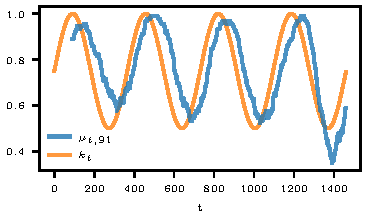
\includegraphics{plots/illustrative_examples/trending_ratio_time_series.pdf}
    \caption{Rolling estimate of the trending ratio over time with window length 91. }\label{fig:trending_ratio_time_series}
    \end{subfigure}%
    \caption{Visualizations for data with a time-varying trending ratio. We defer information on the data generation process of the data in \ref{fig:trending_basic_4q_sample} and \ref{fig:trending_basic_4q_sample_color} to the appendix (see \ref{subsec:app-trending-data-generation}). The trending ratios on the whole data set are $\mu = 0.7577$ and with exclusion area $\diffx < \varepsilon$, $\mu_{1.0} = 0.7712$, respectively. Strong yearly seasonality of the trending ratio becomes visible in Figure~\ref{fig:trending_ratio_time_series}. The green curve $k_t$ shows the probability of $\diffxt$ having the same sign as $\diffyt$ for each time step. The rolling estimates hang back as the windows are backward-looking.}
\end{figure}


In applications, signal data is often not available for all time steps, for example, due to technical problems or delays in data transfer (see the examples in Sections~\ref{sec:application-covid} and~\ref{sec:application-forecasting}).
We refer to time steps, for which either signal or true values or both are unavailable, as missing values.
Data pairs with missing values can be excluded from the computation of the measures so that the time indices with missing values are excluded from $\mathcal{T}$.
In general, the measures can be computed for data with missing values if the missing values do not systematically occur.
Systematic missing values would lead to a biased estimate of the trending ratio, for example, if signal data is omitted in times of high change and thus uncertainty.
In this case, the measures should be computed for the time steps with available data, and the results should be interpreted cautiously.
Thus, inspection of missing data should accompany applications with missing data, for example, through a visual assessment.
In the applications in Sections~\ref{sec:application-covid} and~\ref{sec:application-forecasting}, only a few missing values occur, and we give information on the missing data by inspecting the missing data as lists.

\subsection{Accounting for noise and non-informative small changes}\label{subsec:trending-noise}

The above measures use only the information on a point's quadrant and neglect further details on its location within the quadrant.
However, points close to the zero point have intuitively less explanatory power or are less reliable.
If there is noise or non-systematic effects present in true value or predictions, those points are likely to be driven by noise to a large amount.
That means that the quadrant the point's assignment to a quadrant is driven by noise instead of a systematic trending ability of the signal.

Using an exclusion area around the zero point is a straightforward and highly interpretable extension of the measures of Section~\ref{subsec:trending-measures}.
Points within that zone are neither plotted in the four-quadrant plot nor included in the calculation of the measures.
The exclusion area's shape can be chosen according to the noise characteristics in predictions and true values.
In general, it is likely that the models of predictions have a noise component and should thus be part of the exclusion area.
We denote the measures of Equations~\eqref{eq:acc},~\eqref{eq:accp} and~\eqref{eq:accm} accounting for an exclusion area $e$ by
\begin{align}
    \acceps (\diffx, \diffy, e) &\coloneqq \frac{\sum_{t \in \mathcal{T}} \ind{\diffx \diffy > 0} \ind{(\diffyt, \diffxt) \notin e}}{\sum_{t \in \mathcal{T}} \ind{(\diffyt, \diffxt) \notin e}}\label{eq:acceps}\\
    \accpeps (\diffx, \diffy, e) &\coloneqq \frac{\sum_{t \in \mathcal{T}} \ind{\diffxt \diffyt > 0} \ind{\diffxt > 0, , (\diffyt, \diffxt) \notin e}}{\sum_{t \in \mathcal{T}} \ind{\diffxt > 0, , (\diffyt, \diffxt) \notin e}} \label{eq:accpeps}\\
    \accmeps (\diffx, \diffy, e) &\coloneqq \frac{\sum_{t \in \mathcal{T}} \ind{\diffxt \diffyt > 0} \ind{\diffxt < 0, (\diffyt, \diffxt) \notin e}}{\sum_{t \in \mathcal{T}} \ind{\diffxt < 0, (\diffyt, \diffxt) \notin e}}\label{eq:accmeps}
\end{align}

\todo[inline]{Bsp. für einfache Exclusion area mit rectangle und resulting measures; Bsp. für andere shapes und wie dann $e$ gestaltet wäre}

The measures are then estimators for the probability of trending, given that the change is not in the exclusion area $e$, that is, $P(\diffxrv \diffyrv > 0 | \diffxrv \diffyrv \notin e)$.
The estimators can easily be adapted for various shapes of the exclusion area.
Figure~\ref{fig:trending_4q} visualizes different shapes of the exclusion area.
A rectangularly shaped exclusion area, $e = \{(x, y) \in \R^2: (-\varepsilon_x \leq x \leq \varepsilon_x) \land (-\varepsilon_y \leq y \leq \varepsilon_y) \}$ for $\varepsilon_x, \varepsilon_y > 0$, leaves points out that are small in both components and are thus likely to be driven away from the zero point by noise.
Points where at least the true value or signal is unlikely to be zero are not excluded.
In the example plot, only point 1 is excluded.
An exclusion area along one axis, for example, $e = \{(x, y) \in \R^2: (-\varepsilon_x \leq 0 \leq \varepsilon_x)\}$ for $\varepsilon_x > 0$, removes points in which one of the components could change the sign by a small amount of noise.
This particularly suits signals where small amounts of noise are inevitable.
A cross-shaped exclusion area, $e = \{(x, y) \in \R^2: (-\varepsilon_x \leq x \leq \varepsilon_x) \lor (-\varepsilon_y \leq y \leq \varepsilon_y) \}$ for $\varepsilon_x, \varepsilon_y > 0$, along both axes accounts for likely sign reversal in both components.
For those two methods, points 1 and 7 or 1, 6, and 7 are excluded, respectively.

In addition to these straight shapes, exclusion areas could have more complex shapes, such as ellipses.
Such a shape could, for example, be obtained by using a multivariate normal error model around the zero point and excluding points that exceed a certain likelihood of being produced by chance from the zero point.
These shapes are theoretically appealing, but interpreting the resulting estimators gets complex.
Thus, we use the simple exclusion areas above.

In most applications, it is advisable to determine the exact shape and size of the exclusion area based on domain knowledge or expert opinions.
In addition, the size can also be calculated as a proportion of the total variance or the total range of the data.
A third approach is to visualize the trending ratio for different values of $e$.
Section~\ref{sec:application} contains various examples of such a plot.
As a base approach, we advocate using no exclusion area in the four-quadrant plot as the points do not complicate its interpretation and a $\acceps$-over-$e$ plot to visualize the course of the trending ratio over different exclusion area sizes.


\subsection{The conditional trending plot and confidence intervals based on bootstrapping}\label{subsec:trending-cond-prob}
The above-defined estimators give information on the probabilites $P(\diffxrv \diffyrv > 0 | \diffxrv \diffyrv \notin e)$, $P(\diffxrv \diffyrv > 0 | \diffxrv > 0, \diffxrv \diffyrv \notin e)$ and $P(\diffxrv \diffyrv > 0 | \diffxrv < 0, \diffxrv \diffyrv \notin e)$.
These probabilities draw a general picture but might still be too coarse for local effects.
More insights might be gained by considering the conditional distribution to assess the local trending ability of a prediction.
Whereas it would be possible to build analog measures on other intervals, assessing $P(\diffxrv \diffyrv > 0 | \diffx = x)$ graphically eases the simultaneous evaluation of various intervals.
In addition, the conditional trending plot facilitates the comparison of various methods in a single plot and asymmetries of $P(\diffxrv \diffyrv > 0 | \diffx = x)$ with respect to $x$ in the trending ability can be detected.

A multivariate \acf{kde} facilitates a continuous estimation of $P(\diffxrv \diffyrv > 0 | \diffxrv = x)$ by estimating the components $f_{\diffxrv, \diffyrv}$ and $f_{\diffxrv}$ of
\begin{align*}
P(\diffxrv \diffyrv > 0 | \diffxrv = x) = \begin{cases}
                                              \int_{-\infty}^0 \frac{f_{\diffxrv, \diffyrv}(x, y)}{f_{\diffxrv}(x)} \: \textrm{d} \: y & \text{if } x < 0, \\
                                              \int_{0}^{\infty} \frac{f_{\diffxrv, \diffyrv}(x, y)}{f_{\diffxrv}(x)} \: \textrm{d} \: y & \text{if } x > 0, \\
\end{cases}
\end{align*}
for $x \neq 0$ through a \ac{kde}.
A comprehensive introduction into multivariate \ac{kde} can be found in \textcite{Gramacki2018}, and implementations are available in many programming languages~\parencite[e.g., for  Python in][]{Seabold2010}.
The \ac{kde} yields estimates for $P(\diffxrv \diffyrv > 0 | \diffxrv = x)$ for all values of $x \in \R$.
Note that for kernels with infinite support, for example, the Gaussian kernel, the plot should be limited to the core values of $\diffx$ without outliers to avoid estimates based on small subsets of the data.
Besides the kernel, a bandwidth selector has to be chosen for a multivariate \ac{kde}.
Various methods are available with different strengths and weaknesses.
Figure~\ref{fig:trending-cond-prob-bw} shows the resulting conditional trending plots for the three well-known selectors, rule-of-thumb, cross-validation maximum likelihood, and cross-validation least squares using the \verb|statsmodels| python package~\parencite{Seabold2010}.
While the rule-of-thumb is based only on the covariance matrix, the other two numerically optimize the bandwidth with a hold-one-out least squares or likelihood objective function.
The dashed line shows the theoretical $P(\diffyrv \diffxrv > 0 | \diffxrv = x)$.
The second method, cross-validation least squares, needs long computation times while yielding small or no bandwidth results, even for two relatively small datasets.
The rule-of-thumb and cross-validation maximum likelihood both yield reasonable results at moderate computation times. 
Further examples, including comparisons between methods concerning their trending ability, are available for the applications in Section~\ref{sec:application}.

\begin{figure}
    \centering
    \begin{subfigure}{.48\textwidth}
        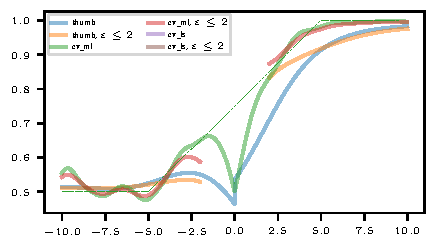
\includegraphics{plots/illustrative_examples/cond_prob_plot_bw_asym_butterfly}
        \caption{First dataset with asymmetric dependence.}
    \end{subfigure}
    \begin{subfigure}{.48\textwidth}
        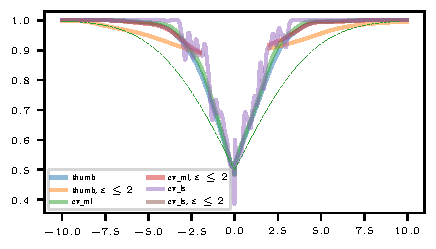
\includegraphics{plots/illustrative_examples/cond_prob_plot_bw_normal}
        \caption{Second dataset. }
    \end{subfigure}
    \caption{Resulting conditional trending plot for different bandwidth selection processes. Cross-validation least squares takes a considerably larger computation time. It does not converge for the first data set and yields a bandwidth too small for the second data set. The rule of thumb is the fastest method but tends to oversmooth. The cross-validation maximum likelihood method yields a more reasonable bandwidth with moderate computation time. }\label{fig:trending-cond-prob-bw}
\end{figure}

Confidence intervals can account for the estimation uncertainty of the measures above.
Bootstrap confidence intervals are a nonparametric technique based on resampling~\parencite[for introductions see][]{Hesterberg2011,Bittmann2021}.
New samples are drawn with replacement from the dataset in bootstrapping and are not based on parametric assumptions as for classical confidence intervals.
The confidence interval is then computed based on the bootstrap samples.
We examine three methods for bootstrapping here: the intuitive percentile and the more sophisticated basic and \ac{bca} method.
In the \textit{percentile} approach, the confidence interval for level $\alpha$ is built directly from the bootstrap estimators' empirical distribution.
The \textit{basic} approach computes the confidence interval based on the non-bootstrapped estimate using the bootstrapped quantile deviations~\parencite{Davison1997}.
The \ac{bca} method modifies the quantiles of the empirical bootstrap distribution by a bias and an acceleration parameter~\parencite{Efron1987}.
Typically, the percentile approach needs larger datasets and provides an easy and fast estimate, while the \ac{bca} is computationally expensive but needs smaller datasets for reasonable confidence intervals.
The basic approach balances those two aims.
We compare the approaches in a small synthetic data study concerning their small-dataset behavior and computation time in Appendix~\ref{sec:appendix}.
For small datasets, the \ac{bca} holds the confidence level also for small data sets with a negligibly higher computation time than the other approaches.
Thus, we use the \ac{bca} method for the confidence intervals in the applications in Section~\ref{sec:application}.

The sample is assumed to be independent and identically distributed in standard bootstrapping.
Thus, before applying bootstrapping methods, the strength of sequential dependence should be inspected, for example, by analyzing the autocorrelation and partial autocorrelation.
The simple bootstrapping methods above do not account for serial dependence. 
Bootstrapping focusing on time series data is covered in~\textcite{Hardle2003,Kreiss2012}, for example.

\subsection{Probabilistic Evaluation}

\todo{Schreiben}
